% This version of CVPR template is provided by Ming-Ming Cheng.
% Please leave an issue if you found a bug:
% https://github.com/MCG-NKU/CVPR_Template.

% \documentclass[review]{cvpr}
\documentclass[final]{cvpr}

\usepackage{times}
\usepackage{epsfig}
\usepackage{graphicx}
\usepackage{amsmath}
\usepackage{amssymb}

% Include other packages here, before hyperref.

% If you comment hyperref and then uncomment it, you should delete
% egpaper.aux before re-running latex.  (Or just hit 'q' on the first latex
% run, let it finish, and you should be clear).
\usepackage[pagebackref=true,breaklinks=true,colorlinks,bookmarks=false]{hyperref}


\def\confYear{CVPR 2021}
%\setcounter{page}{4321} % For final version only


\begin{document}

%%%%%%%%% TITLE
\title{The Report of the Assignment 1:\\Implementing and Reproducing Elastic Weight Consolidation}

\author{Seungmin Lee\\
Seoul National University\\
{\tt\small dltmdals14@snu.ac.kr}
}

\onecolumn
\maketitle


%%%%%%%%% BODY TEXT
\section{Introduction}
Elastic Weight Consolidation (EWC)~\cite{ewc} is a pioneering work that tackles continual learning problems. Even though many researchers have already validated EWC in their papers, we implement and reproduce EWC and compare it with L2 regularization. We conduct two experiments using CIFAR100~\cite{cifar} and MNIST~\cite{mnist}: (a) hyperparameter searching, (b) comparing the effectiveness of EWC, L2 regularization, and no regularization. In these experiments, we learn the following three lessons. First, both regularization can alleviate \textit{catastrophic forgetting}. Second, the optimal hyperparameters can be highly different between datasets. For example, the optimal hyperparameter for CIFAR100 is 1.0. On the other hand, the optimal value is 100.0 for MNIST. Third, on simple datasets such as MNIST, EWC can be less effective than L2 regularization. 

\section{Methods}\label{method}
In this section, we summarize the methods that we implement for this assignment. Because our primary concerns are regularization-based continual learning methods, the loss functions have the same form as follows:
\begin{align}
	\mathcal{L}(\theta) = \mathcal{L}_{CE}(\theta) + \lambda\mathcal{L}_{reg}(\theta, \theta_T)
\end{align}
where $\theta$ and $\theta_T$ denote the current model weights and the previous weights after training on task $T$, repectively, and $lambda$ is the hyperparameter that balances the classification loss $\mathcal{L}_{CE}$ and the regularization loss $\mathcal{L}_{reg}$. The regularization loss term $\mathcal{L}_{reg}$ makes the difference between EWC, L2 regularization, and no regularization.

EWC alleviates catastrophic forgetting by preventing $\theta$ far away from the important weights of $\theta_{T}$ because $\theta_{T}$ encodes the knowledge for solving the previous tasks. EWC estimates the importance of each weight by calculating Fisher Information Matrix. Therefore, the regularization term of EWC~\cite{ewc} is 
\begin{align}
	\mathcal{L}_{reg}(\theta, \theta_T) = \sum_i F_i(\theta_i - \theta_{T,i})^2
\end{align}
where $F$ denotes the Fisher information matrix, $i$ is an index of each parameters. For efficiency, EWC adopts the diagonal approximation of the Fisher information matrix.

L2 regularization uses the following equation as its regularization term:
\begin{align}
	\mathcal{L}_{reg}(\theta, \theta_T) = \sum_i(\theta_i - \theta_{T,i})^2.
\end{align}
We can interpret that L2 regularization does not consider the importance of each weight. We use L2 regularization to validate whether the EWC's importance estimation is helpful or not. No regularization or vanilla training does not utilize $L_{reg}$. 

\section{Experiments}
In this section, we describe the experiment settings and their results. First, we conduct experiments for finding the optimal value of $\lambda$ used for balancing $\mathcal{L}_{CE}$ and $\mathcal{L}_{reg}$. In the second experiment, we compare the three methods described in the section~\ref{method}.

\subsection{Hyperparameter Searching}

\begin{figure}[t]
    \centering
	\begin{tabular}{c@{\hskip0.5cm}c}
		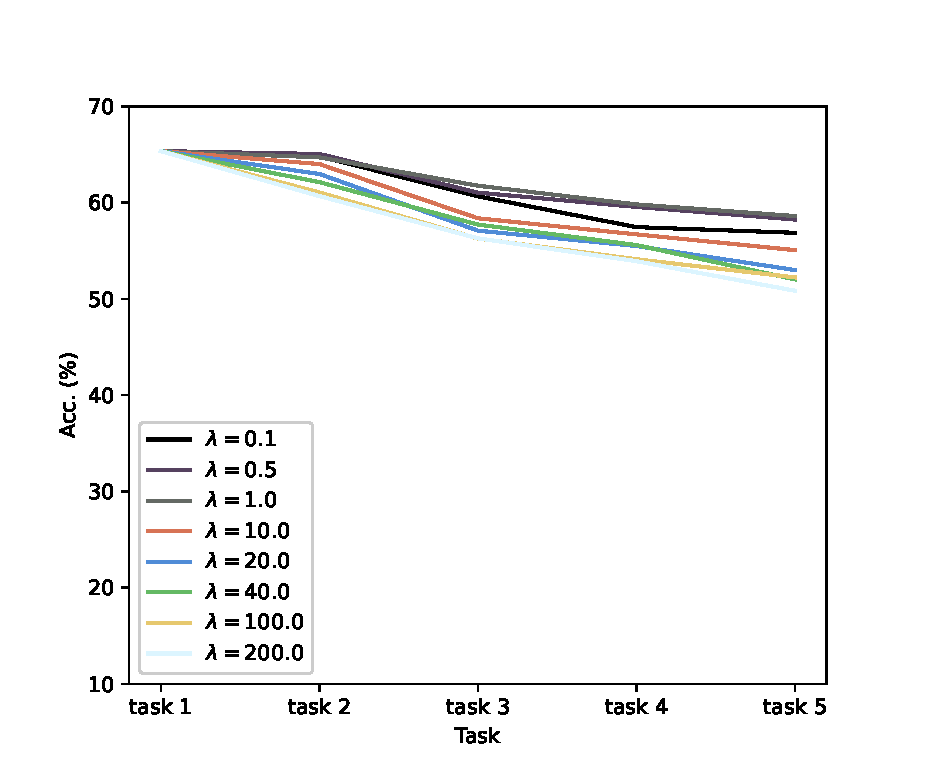
\includegraphics[width=0.45\textwidth]{resources/ewc_CIFAR.eps}&%	
        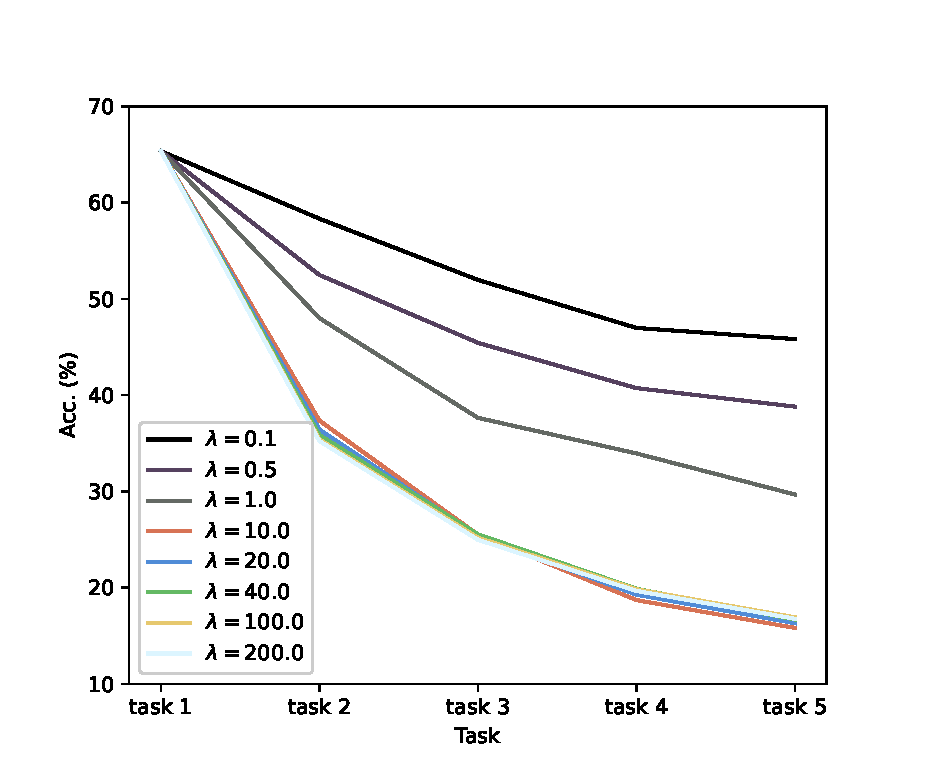
\includegraphics[width=0.45\textwidth]{resources/l2_CIFAR.eps}\\%
        (a) EWC CIFAR100 & (b) L2 CIFAR100\\
        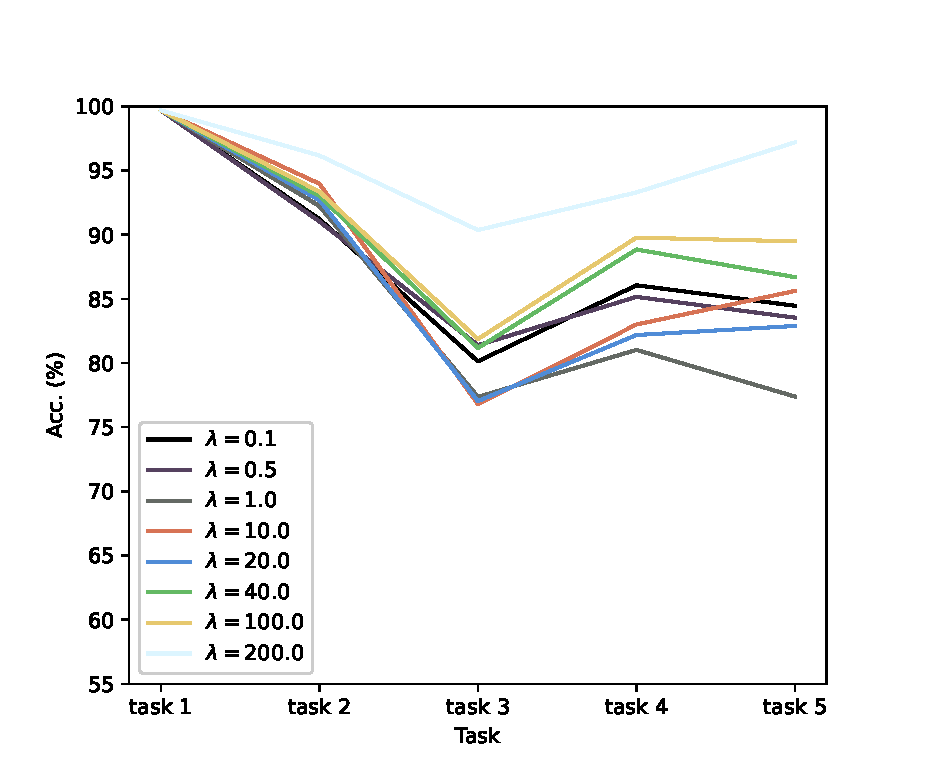
\includegraphics[width=0.45\textwidth]{resources/ewc_MNIST.eps}&%	
        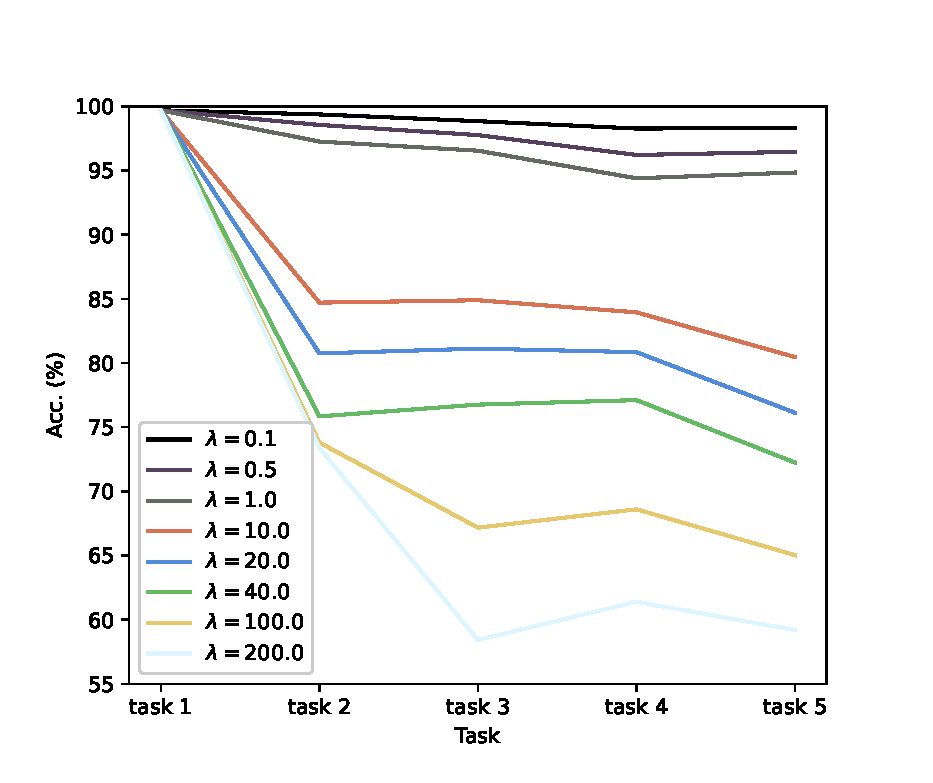
\includegraphics[width=0.45\textwidth]{resources/l2_MNIST.eps}\\%
		(c) EWC MNIST  & (d) L2 MNIST \\
	\end{tabular}\vspace{0.2cm}
	\caption{some captions}
	\label{fig:tsne}
	% \vspace{-0.4cm}
\end{figure}

\begin{figure}[t]
    \centering
	\begin{tabular}{c@{\hskip0.5cm}c}
		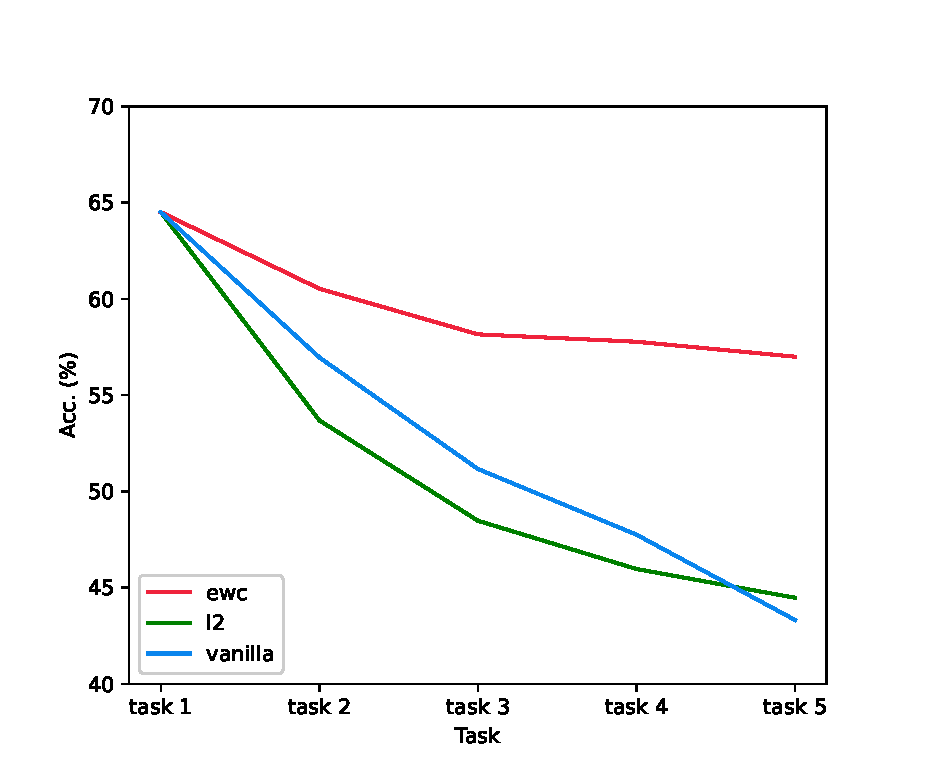
\includegraphics[width=0.45\textwidth]{resources/comp_CIFAR.eps}&%	
        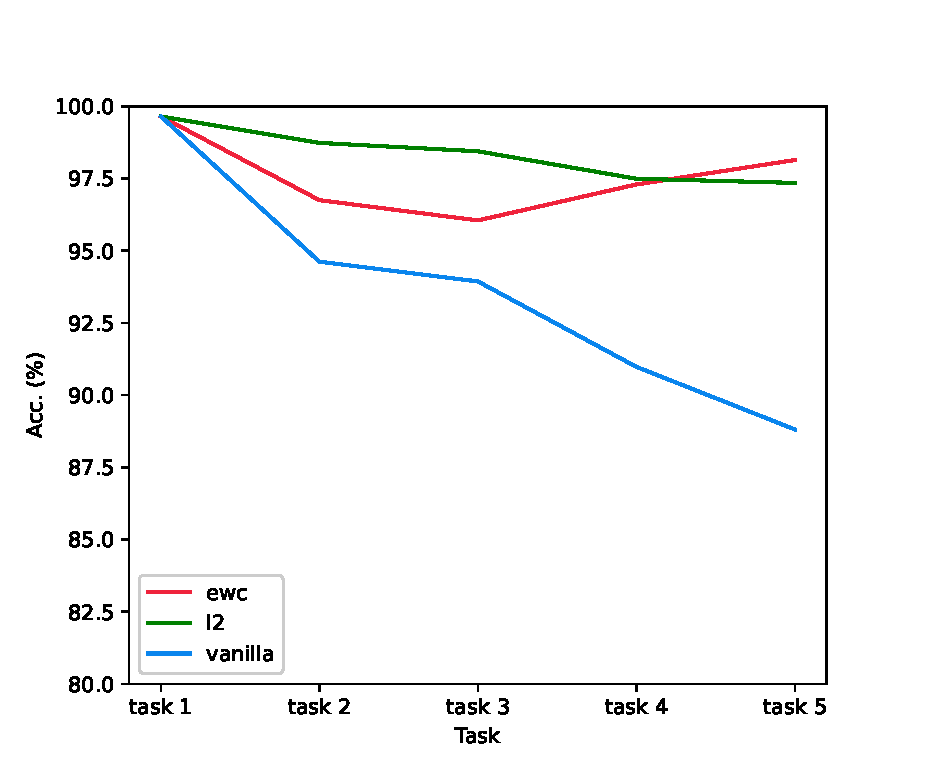
\includegraphics[width=0.45\textwidth]{resources/comp_MNIST.eps}\\%
        (a) Comparing on CIFAR100 & (b) Comparing on MNIST\\
	\end{tabular}\vspace{0.2cm}
	\caption{some captions}
	\label{fig:tsne}
	% \vspace{-0.4cm}
\end{figure}


{\small
\bibliographystyle{ieee_fullname}
\bibliography{egbib}
}

\end{document}
